\documentclass[reprint, english, nofootinbib]{revtex4-2}

\usepackage{graphicx}
\usepackage{subfig}
\usepackage[colorlinks=true,urlcolor=blue,citecolor=blue]{hyperref}
\usepackage{physics}
\usepackage{amsmath}
\usepackage{amssymb}
\usepackage{amsbsy}
\usepackage{subfig}
\usepackage{blindtext}
\usepackage{tikzducks}
\usepackage{tikz}
\usepackage{pgfplots}
\usepackage{listings}

\graphicspath{{../figs/}}


\begin{document}
\title{Solving partial differential equations with neural networks}
\author{Nicholas Karlsen}
\affiliation{University of Oslo}
\author{Thore Espedal Moe}
\affiliation{University of Oslo}
\date{\today}

\begin{abstract}
    An abstract abstract
\end{abstract}

\maketitle

\section{Introduction}

\section{Theory \& Methods}

\subsection{Solving Differential Equations with Neural Networks}
\noindent
In general, a ordinary differential equation (ODE) may be written in the form
\begin{equation}
    F \qty[x, u(x), u'(x), u''(x), \dots, g^{(n)}(x)] = 0
\end{equation}    
where $u(x)$ denotes the solution of the ODE. One may then propose a trial solution $u_t(x,P)$ in the form
\begin{equation}
    u_{t}(x, P) = u_{bc}(x) + u_{nn}(x)N(x, P) 
\end{equation}
where $u_{bc}(x), u_{nn}(x)$ are functions which enforce the boundary conditions of the ODE and $N(x, P)$ is a neural network with independent variables denoted by $P = \{W\},\{\pmb b\}$, the weights and biases in the network respectively.. In order to optimize $N(x, P)$ such that $u_t(x)$ yields a solution of the ODE, we define the cost function by the $L^2$ norm of $F$ as
\begin{equation}
    \mathcal C\qty[u\qty(x)] = \frac{1}{N} \sum_{i=1}^{N}\qty(F\qty[x, u(x_i), u'(x_i), \dots, u^{(n)}(x_i)])^2
\end{equation}
where we have discretized as $x \rightarrow \{x_1, x_2 ,\dots, x_{N}\}$. We can then construct a Feed-Forward Neural network with $L-1$ hidden layers which for each itteration updates the weights and biases of the network wrt. to the current trial solution $u_t(x)$ evaluated with the cost function. See \cite{4155_project_2}

As a note, for some network architectures it is possible to obatin fairly simple derivatives of these types of cost-functions with respect to the network parameters, see e.g. \cite{Lagaris_1998}. However, it is in general quite burdensome to set up the network-derivatives by hand. Thus a major boost for the use of Neural Networks in solving differential equations comes from the advent of Automatic Differentiation, which by tracking the elementary operations performed in the network computations is capable of accurately and automatically producing the sought-after gradients. In the present work we rely on the autograd-functionality of PyTorch, to produce all necessary derivatives.

\subsection{The Heat Equation}

As our first example we investigate the application of Neural Networks for solving the so-called Heat Equation. In physics, the Heat equation models how the temperature of some material $u\qty(\pmb r, t)$ evolves over time by the partial differential equation (PDE)
\begin{equation}
    \pdv{u}{t} = c^2\nabla^2 u 
\end{equation}
where $c^2$, the thermal diffusivity is a material dependent constant. 
This may be reduced to a one dimensional problem, modelling i.e a thin, insulating wire of length $L$ as
\begin{equation}\label{eqn: 1D heat eqn}
    \pdv{u}{t} = \pdv[2]{u}{x}
\end{equation}
where we have also for simplicity set $c^2 = 1$. We may then solve this analytically with boundary conditions $u\qty(0, t) = u\qty(L,t) = 0$ and initial condition $u(x, 0) = f(x)$.

\subsubsection{Solving the Heat Equation analytically}
\noindent 

We start by making the assumption that $u(x, t)$ is separable, giving 
\begin{equation}
    u(x, t) = F(x) \cdot G(t)
\end{equation}
which lets us rewrite Eqn.~\ref{eqn: 1D heat eqn} to the form
\begin{equation}
    F \cdot \pdv{G}{t} = \pdv[2]{F}{x} \cdot G
\end{equation}
which may be expressed as
\begin{equation}
    \frac{\dot G}{G} = \frac{F^{''}}{F} = k
\end{equation}
where $k$ is some constant. We further have that the boundary conditions may only be satisfied for $k <  0$, so we set $k = -\rho^2$ and write
\begin{equation}
    F^{''} + \rho F = 0 \quad \quad \dot G + \rho^2G = 0
\end{equation}
starting with the spatial equation, we have a general solution in the form 
\begin{equation}
    F(x) = c_1 \cos(\rho x) + c_2 \sin(\rho x)
\end{equation}
where $c_1 = 0$ is fixed by $u(0, t) = $. Similarly, $u(L, t) = 0$ imposes the requirement $\sin(\rho x) = 0$ which is satisfied by setting $\rho = n\pi/L$, yielding a discrete spectrum of solutions
\begin{equation}
    F_n(x) = \sin\qty(\frac{n\pi x}{L})
\end{equation}
where we omit the constant $c_1$, which we will include later in $G(t)$. 

We then move on to the temporal part, $G(t)$, which we write as
\begin{equation}
    \dot G = -\rho^2G
\end{equation}
which we immediately recognize as having a general solution
\begin{equation}
    G(t) = c_n e^{-n^2\pi^2 t / L^2}
\end{equation}
Thus, $u(x, t)$ is solved by a superposition of the discrete set of eigenfunctions
\begin{equation}
    u_n\qty(x, t) = \sum_{n=1}^{\infty} c_n \sin\qty(\frac{n\pi x}{L}) e^{-n^2\pi^2 t / L^2}
\end{equation}
with initial condition
\begin{equation}
    u(x, 0) = \sum_{n=1}^{\infty} c_n \sin\qty(\frac{n\pi x}{L}) = f(x)
\end{equation}
a Fourier series. Thus, the coefficients $c_n$ are determined by the integral
\begin{equation}
    c_n = \frac{2}{L}\int_0^L \dd x \, f(x) \sin\qty(\frac{n\pi x}{L})
\end{equation}
if we set the initial condition $f(x) = \sin(\pi x)$ and fix $L = 1$, we get coefficients
\begin{equation}
    c_n = 2\int_0^1 \dd x \, \sin(\pi x) \sin(n\pi x) = 1
\end{equation}
we thus have an analytical solution for the Heat equation with boundary conditions $u(0, t) = u(L, t) = 0$, $L = 1$, and initial condition $u(x, 0) = \sin(\pi x)$ as
\begin{equation}
    u(x, t) = \sin\qty(\pi x) e^{-\pi^2 t}
\end{equation}
a plot of which for $t \in [0, 1]$ is shown in Fig.~\ref{fig: heat eqn analytic}.
\begin{figure}[h!tb]
    \center
    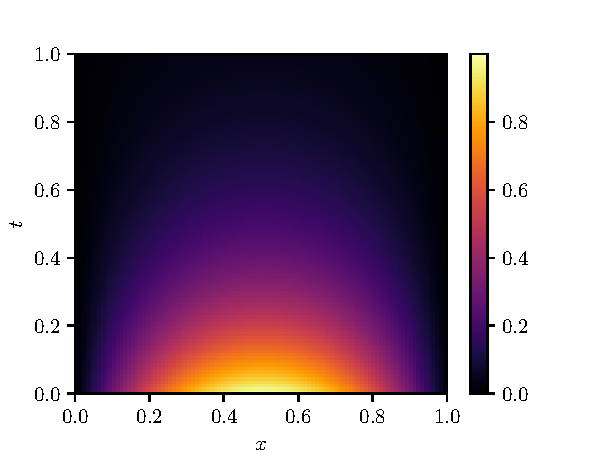
\includegraphics[width=.8\columnwidth]{heat_eqn_analytic.pdf}
    \caption{\label{fig: heat eqn analytic}}
\end{figure}

\subsubsection{Solving the Heat Equation through a simple Finite-Difference scheme}

While we in this case were able to obtain a simple analytic solution to the differential equation, that is generally not possible for most PDEs so numerical methods must be used instead. The simplest, though neither the most accurate nor the most stable, class of numerical methods for solving PDEs are the so-called explicit finite-difference schemes. The main idea consists of dividing the computational domain into a set of grid points, and discretizing the differential equations to obtain relations between the function values at those grid-points. 

The distinction between explicit and implicit schemes is, of course, that with an explicit scheme the values at the next grid points can be explicitly calculated from the previous grid points so that given the boundary conditions one obtains a rule for calculating the function values of the whole domain one step at the time. Oppositely, implicit schemes give the value at a grid-point as a function of both that grid-point's value and the values of the previous grid-points thus requiring the (usually numerical) solution of a linear system of equations for each grid-point. The benefit of implicit methods is that they usually have more lax restrictions on how the grid-points must be spaced in order to maintain stability of the solution.

For the case at hand one rewrites %% u(x_i,t_i) = (u(x_i-1,t_i-1) - 2*u(x_i,t_i-1) + u(x_i+1,t_i-1) * dt/dx2. First setup grid, then discretize du/dx2 into (u(x_i-1)-2*u(x_i) + u(x_i+1))/dx2 and du/dt = (u(t_i) - u(t_i-1))/dt. Move around these two equations and you get the formula. Can be rewritten as a matrix equation: u_vector(t_i+1) = tridiagonal matrix * u_vector(t_i) * dt/dx2 with zero-padding on top and bottom row to accomodate the BC. Stability criterion dt/dx2 <= 1/2, if not fulfilled round-off errors will cause the solution to explode. 



\subsubsection{Solving the Heat Equation with Neural Networks}
\noindent
We now turn to the use of a neural network as an alternative method for obtaining the solution of the Heat Equation. We start by re-writing Eqn.~\ref{eqn: 1D heat eqn} to the form
\begin{equation}
    \pdv{u}{t} - \pdv[2]{u}{x} = 0
\end{equation}
which gives rise to the cost function 
\begin{equation}
    \mathcal C\qty[u\qty(x, y)] = \frac{1}{N}\sum_{i=1}^N \qty(\pdv{u}{t} - \pdv[2]{u}{x})^2
\end{equation}
setting the boundary conditions $u(0, t) = u(L, t) = 0$ and initial condition $u(x, 0) = \sin(\pi x)$, we then have a trial solution in the form
\begin{equation}
    u_t(x, t, P) = \qty(1 - t)\sin(\pi x) + x(1 - x)t N(x, t, P)
\end{equation}

\begin{figure}[h!tb]
   \center
   


\tikzset{every picture/.style={line width=0.75pt}} %set default line width to 0.75pt        

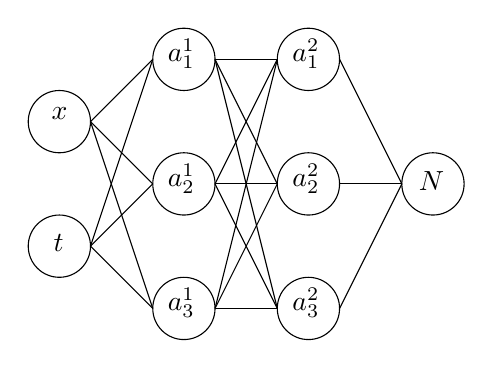
\begin{tikzpicture}[x=0.75pt,y=0.75pt,yscale=-1,xscale=1]
%uncomment if require: \path (0,695); %set diagram left start at 0, and has height of 695

%Shape: Ellipse [id:dp613538016915602] 
\draw   (80,265) .. controls (80,256.72) and (86.72,250) .. (95,250) .. controls (103.28,250) and (110,256.72) .. (110,265) .. controls (110,273.28) and (103.28,280) .. (95,280) .. controls (86.72,280) and (80,273.28) .. (80,265) -- cycle ;
%Shape: Ellipse [id:dp15712636391006307] 
\draw   (80,205) .. controls (80,196.72) and (86.72,190) .. (95,190) .. controls (103.28,190) and (110,196.72) .. (110,205) .. controls (110,213.28) and (103.28,220) .. (95,220) .. controls (86.72,220) and (80,213.28) .. (80,205) -- cycle ;
%Shape: Ellipse [id:dp8164179950038163] 
\draw   (140,175) .. controls (140,166.72) and (146.72,160) .. (155,160) .. controls (163.28,160) and (170,166.72) .. (170,175) .. controls (170,183.28) and (163.28,190) .. (155,190) .. controls (146.72,190) and (140,183.28) .. (140,175) -- cycle ;
%Shape: Ellipse [id:dp47375219812723146] 
\draw   (140,235) .. controls (140,226.72) and (146.72,220) .. (155,220) .. controls (163.28,220) and (170,226.72) .. (170,235) .. controls (170,243.28) and (163.28,250) .. (155,250) .. controls (146.72,250) and (140,243.28) .. (140,235) -- cycle ;
%Shape: Ellipse [id:dp712019427556807] 
\draw   (140,295) .. controls (140,286.72) and (146.72,280) .. (155,280) .. controls (163.28,280) and (170,286.72) .. (170,295) .. controls (170,303.28) and (163.28,310) .. (155,310) .. controls (146.72,310) and (140,303.28) .. (140,295) -- cycle ;
%Straight Lines [id:da6435868346848231] 
\draw    (110,205) -- (140,175) ;
%Straight Lines [id:da08712551076022779] 
\draw    (110,265) -- (140,235) ;
%Straight Lines [id:da18860583656122687] 
\draw    (110,265) -- (140,175) ;
%Straight Lines [id:da267566031093317] 
\draw    (110,265) -- (140,295) ;
%Straight Lines [id:da6453145574577351] 
\draw    (110,205) -- (140,295) ;
%Straight Lines [id:da9129290543985238] 
\draw    (110,205) -- (140,235) ;
%Shape: Ellipse [id:dp31900160827767665] 
\draw   (200,175) .. controls (200,166.72) and (206.72,160) .. (215,160) .. controls (223.28,160) and (230,166.72) .. (230,175) .. controls (230,183.28) and (223.28,190) .. (215,190) .. controls (206.72,190) and (200,183.28) .. (200,175) -- cycle ;
%Shape: Ellipse [id:dp21066050092203037] 
\draw   (260,235) .. controls (260,226.72) and (266.72,220) .. (275,220) .. controls (283.28,220) and (290,226.72) .. (290,235) .. controls (290,243.28) and (283.28,250) .. (275,250) .. controls (266.72,250) and (260,243.28) .. (260,235) -- cycle ;
%Shape: Ellipse [id:dp8190479437064692] 
\draw   (200,235) .. controls (200,226.72) and (206.72,220) .. (215,220) .. controls (223.28,220) and (230,226.72) .. (230,235) .. controls (230,243.28) and (223.28,250) .. (215,250) .. controls (206.72,250) and (200,243.28) .. (200,235) -- cycle ;
%Shape: Ellipse [id:dp9436580210127415] 
\draw   (200,295) .. controls (200,286.72) and (206.72,280) .. (215,280) .. controls (223.28,280) and (230,286.72) .. (230,295) .. controls (230,303.28) and (223.28,310) .. (215,310) .. controls (206.72,310) and (200,303.28) .. (200,295) -- cycle ;
%Straight Lines [id:da5770582110402913] 
\draw    (170,175) -- (200,175) ;
%Straight Lines [id:da378598346323751] 
\draw    (170,175) -- (200,235) ;
%Straight Lines [id:da045787154766960936] 
\draw    (170,175) -- (200,295) ;
%Straight Lines [id:da10461814863080832] 
\draw    (170,295) -- (200,175) ;
%Straight Lines [id:da18820240172871194] 
\draw    (170,295) -- (200,235) ;
%Straight Lines [id:da7563044436713307] 
\draw    (170,295) -- (200,295) ;
%Straight Lines [id:da9591828994155338] 
\draw    (170,235) -- (200,295) ;
%Straight Lines [id:da039530432138651816] 
\draw    (170,235) -- (200,235) ;
%Straight Lines [id:da03185694587768484] 
\draw    (170,235) -- (200,175) ;
%Straight Lines [id:da6835990243055697] 
\draw    (230,235) -- (260,235) ;
%Straight Lines [id:da4490575310089562] 
\draw    (230,295) -- (260,235) ;
%Straight Lines [id:da36571324995783205] 
\draw    (230,175) -- (260,235) ;

% Text Node
\draw (91,258) node [anchor=north west][inner sep=0.75pt]    {$t$};
% Text Node
\draw (90,197) node [anchor=north west][inner sep=0.75pt]    {$x$};
% Text Node
\draw (146,164) node [anchor=north west][inner sep=0.75pt]    {$a^{1}_{1}$};
% Text Node
\draw (146,224) node [anchor=north west][inner sep=0.75pt]    {$a^{1}_{2}$};
% Text Node
\draw (146,284) node [anchor=north west][inner sep=0.75pt]    {$a^{1}_{3}$};
% Text Node
\draw (206,164) node [anchor=north west][inner sep=0.75pt]    {$a^{2}_{1}$};
% Text Node
\draw (267,228) node [anchor=north west][inner sep=0.75pt]    {$N$};
% Text Node
\draw (206,224) node [anchor=north west][inner sep=0.75pt]    {$a^{2}_{2}$};
% Text Node
\draw (206,284) node [anchor=north west][inner sep=0.75pt]    {$a^{2}_{3}$};


\end{tikzpicture}
 
   \caption{Possible network structure of a Feed-Forward network with input $(x,t)$ and 2 hidden layers each with 3 neurons with activations denoted as $a^l_j$ and a single output $N$.}
\end{figure}


\subsection{A Nonlinear System of Ordinary Differential Equations for Finding Eigenvalues and Eigenvectors of Real Symmetric Matrices}

For our second example, we investigate the use of neural networks for the solution of a nonlinear system of ordinary differential equations. The particular use case is the system of differential equations presented by \cite{Yi_2004} for finding the largest eigenvalue $\lambda_{1}$ and corresponding eigenvector $\mathbf{v}_1$ of an $N \times N$ real and symmetric matrix $\mathbf{A}$:

\begin{equation}
\label{eq:yi_eq}
\frac{d \mathbf{x}(t)}{dt} = - \mathbf{x}(t) + [\mathbf{x}(t)^T \mathbf{x} \mathbf{A} - (1 - \mathbf{x}(t)^T \mathbf{x}(t)) \mathbf{I} ] \mathbf{x}(t)
\end{equation}

where $\mathbf{x}(t)$ is a $ 1 \times N$ column vector and $\mathbf{I}$ is an $N \times N$ identity matrix. In \cite{Yi_2004} it is shown that for any initial vector $\mathbf{x}(0)$ which is not orthogonal to eigenspace of the eigenvalue $\lambda_1$, the solution $\mathbf{x}(t)$ of the system \ref{eq:yi_eq} as $t$ goes to infinity converges to an eigenvector $\mathbf{v}_1$ corresponding to the largest eigenvalue of $\mathbf{A}$. It is further shown in \cite{Yi_2004} that replacing $\mathbf{A}$ with $\mathbf{-A}$ in \ref{eq:yi_eq} makes the solution converge instead to an eigenvector of the smallest eigenvalue $\lambda_N$ belonging to $\mathbf{A}$, so long as the initial vector $\mathbf{x}(0)$ is not orthogonal to the eigenspace of that eigenvalue $\lambda_N$. Finally, they give the following recipe for obtaining the eigenvalue from the converged eigenvector:

\begin{equation}
\label{eq:yi_eigenvalue}
\lambda = \frac{\mathbf{v}^T \mathbf{A} \mathbf{v}}{\mathbf{v}^T \mathbf{v}}
\end{equation}
which follows immediately from the definition of eigenvectors and eigenvalues.

Thus, given a real and symmetric matrix, the largest and smallest eigenvalues along with their corresponding eigenvectors can easily obtained from solving \ref{eq:yi_eq} with an appropriate initial vector $\mathbf{x}(0)$. Now, in order to obtain the remaining eigenvalues and eigenvectors one could in principle apply a deflation technique, like Hotelling's or Wielandt's deflation \cite{Saad_2011} \cite{Roberts}, to the matrix $\mathbf{A}$ and repeat the process for the deflated matrix $\mathbf{A}_D$. That is, however, beyond the scope of our present work; and furthermore, non-trivial numerical issues might be expected to arise in such repeated solutions of \ref{eq:yi_eq}.

\subsubsection{Solution through the Forward-Euler Method}

The authors of \cite{Yi_2004} presented the equation \ref{eq:yi_eq} in the context of Recurrent Neural Networks (RNN), where it describes the dynamics of a certain class of such networks. RNNs are outside our current areas of expertise; however, to the best of our knowledge, the simplest RNN that obeys the dynamics prescribed by \ref{eq:yi_eq} should be completely equivalent to the following explicit integration method (Forward-Euler):

\begin{equation}
\label{eq:yi_euler}
\mathbf{x}(t_{i+1}) = \mathbf{x}(t_i) + \frac{d \mathbf{x}(t_i)}{dt}  dt
\end{equation}
where $dt = t_{i+1} -t_{i}$ is a suitably small time-step,  $\frac{d \mathbf{x}(t_i)}{dt}$ is equation \ref{eq:yi_eq} evaluated at $t=t_i$, and the iterations are started from some initial vector $\mathbf{x}(0)$.

This is, in any case, the simplest numerical integration scheme for solving equation \ref{eq:yi_eq}, and is what we will be using to compare our Neural Network-based solutions with.

\subsubsection{Solution through Neural Networks}

The procedure for solving equation \ref{eq:yi_eq} with a Neural Network is very much the same as for the Heat Equation. First a trial solution satisfying the initial conditions is constructed, in this case we use:

%% TRIAL FUNCTION

Then the cost-function to be optimized is defined, in this case as:

%% COST FUNCTION

Finally the derivatives of the cost-function with respect to the network parameters are computed, and the network parameters are updated:

%% UPDATE

The only real change from the case of the Heat Equation is that the network now must produce $N$ outputs for each input $t$, as opposed to one output for each pair $x,t$ of inputs.


\section{Results \& Discussion}

\subsection{The Heat Equation}

\subsection{The Eigen-problem}

\section{Conclusion}

\onecolumngrid
\bibliography{bibfile}
\twocolumngrid

\end{document}